\subsection{Random Walks}
\subsubsection{Classical Random Walk}
Before discussing quantum random walks, I will first motivate their design using the example of a classical random walk on a discrete number line.
In the classical random walk, a walker (often described as being somewhat inebriated) is constrained to moving up and down a discrete number line, starting their walk at the origin.
To determine whether to take a step to the left (-1) or the right (+1), the walkers flips an unbiased coin, moving to the right if the coin lands on heads and to the left if the coin lands on tails. 
The process is can be repeated over and over until a desired stopping point is reached, after a given number of coin flips, or until the walker has reached a specific destination, such as their house in the case of the inebriated walker.
The walk can also continue on forever and in this limit, the walker will reach every point on the number line.
The probability distribution describing the probability of the walker being in any given position away from the origin is given by a binomial distribution, shown in orange in Figure \ref{fig:discVSclass} for 100 coin flips. 

\subsubsection{Quantum Random Walk}
With the classical random walk model in mind, we are now in a position to "quantise" it into the \emph{quantum random walk}.
In our walker system, we can divide the overall Hilbert space of the QW, $\mathcal{H}$, into two subspaces, the coin subspace $\mathcal{H}_C$ and the position subspace of the walker $\mathcal{H}_W$. 
\begin{equation}
    \mathcal{H} = \mathcal{H}_C \otimes \mathcal{H}_W.
\end{equation}
We note that whilst we do not place any constraints on the size of $\mathcal{H}_W$, we choose $dim(\mathcal{H}_C) = 2$, which is the natural thing to do when quantising our classical walk since the classical coin has two possible states. 
To aid distinguishability between coin states and position states, we write that
\begin{align}
    \langle\mathcal{H}_C\rangle &= \{\ket{\uparrow}, \ket{\downarrow}\}\\
    \langle\mathcal{H}_W\rangle &= \{\ket{k} | k\in\mathbb{Z}\},
\end{align}
where $\langle U \rangle$ denotes a set of vectors which span $U$. 
Therefore, the states $\ket{\uparrow}, \ket{\downarrow}$ take the place of heads and tails on our quantum "coin". 
Having defined the Hilbert space within which the walk will be conducted, we can now define operators within our space that will dictate how the QW will proceed. We first define the "coin flip" operator $C\in \mathcal{H}_C$. 
There are several choices for $C$, details of which can be found here \cite{Tregenna2003}. 
As detailed in \cite{Tregenna2003}, for walks on a line, if we restrict ourselves to choosing an unbiased coin with real coefficients the Hadamard coin
\begin{align}
    C &= \frac{1}{\sqrt{2}}\Big[
    \ket{\uparrow}\bra{\uparrow} +
    \ket{\uparrow}\bra{\downarrow} +
    \ket{\downarrow}\bra{\uparrow} -
    \ket{\downarrow}\bra{\downarrow}\Big]\\
    &= \frac{1}{\sqrt{2}}\Big[(\ket{\uparrow} + \ket{\downarrow})\bra{\uparrow} +
    (\ket{\uparrow} - \ket{\downarrow})\bra{\downarrow}\Big]
\end{align}
is the only choice of coin available. 
Equation (5) makes obvious the action of $C$; if the coin state is $\ket{\uparrow}$ then it becomes an equal superposition of $\ket{\uparrow} + \ket{\downarrow}$, if the coin state is in $\ket{\downarrow}$ then we get an equal superposition of $\ket{\uparrow} - \ket{\downarrow}$. 
These two equal superpositions are often denoted as $\ket{+}$ and $\ket{-}$ respectively.\newline
We then define our shift operator $S \in \mathcal{H}$ which allows the position of our walker to change, dependent on the state of the coin.
\begin{equation}
    S = \sum_k \ket{\uparrow}\bra{\uparrow} \otimes \ket{k + 1}\bra{k} + \ket{\downarrow}\bra{\downarrow} \otimes \ket{k - 1}\bra{k}.
\end{equation}
Again, this representation of $S$ makes manifest its effect on our walker. 
If the coin is in the $\ket{\uparrow}$, then we take a step in the +1 direction, if in the $\ket{\downarrow}$ then we take a step in the -1 direction. 
The probability distribution of such a walk is plotted in Fig \ref{fig:discVSclass}, where the initial coin state is $\ket{\downarrow}$, and is compared to a classical random walk.\newline

\begin{figure}
    \centering
    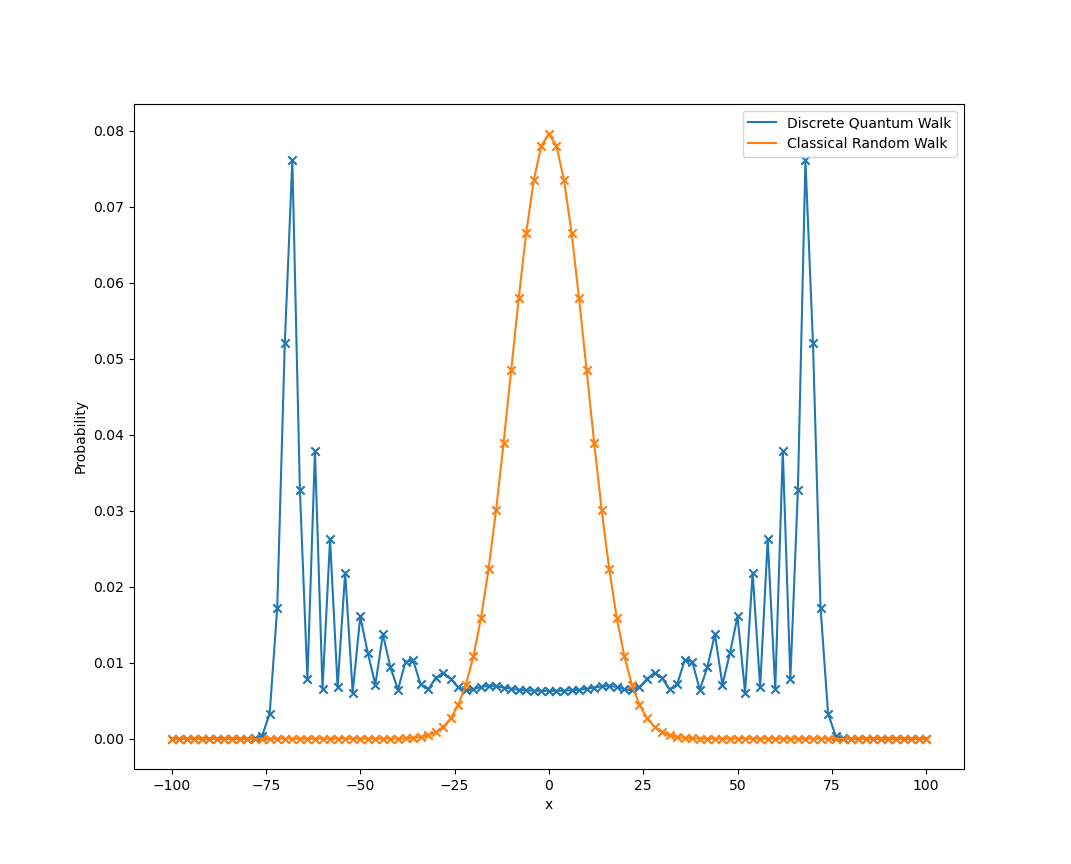
\includegraphics[width = 0.9\textwidth]{Discrete vs Classical Walk.png}
    \caption{A comparison between the classical and quantum walk on a line. The quantum walk is initially in the $\ket{\downarrow}$ state in the coin subspace of the walk.}
    \label{fig:discVSclass}
\end{figure}

Whilst the above choice of $S$ is the most common on the number line, it is also possible to define an alternative choice of shift operator,
\begin{equation}
    \tilde{S} = \sum_k \ket{\uparrow}\bra{\uparrow} \otimes \ket{k}\bra{k} + \ket{\downarrow}\bra{\downarrow} \otimes \ket{k + 1}\bra{k}.
\end{equation}
Th subtle difference between $\tilde{S}$ and $S$ is that $\tilde{S}$ can only move in the $+1$ direction of the number line and has no "left moving" part, so to speak. 
This means that $\tilde{S}$ is restricted to the non-negative integers and unlike $S$, can occupy all $\ket{x}$ for $0\leq x\leq T$, where $T$ is the number of time steps in our QW.